\documentclass{article}
\usepackage{lmodern}
\usepackage[T1]{fontenc}
\usepackage[english,activeacute]{babel}
\usepackage{mathtools}
\usepackage{biblatex}
\usepackage{csquotes}
\usepackage{graphicx}

\setcounter{tocdepth}{5}
%\setcounter{secnumdepth}{5}

\title{User Behavior Analysis in Campus Area Networks through Kohonen Self Organizing Feature Maps}

\author{Nelson Victor Cruz Hern\'andez }

\date{May 2017}

\begin{document}

\maketitle

\section{Introduction} % level 1
Inbounds

\subsection{Background} % level 2

\subsection{Justification} % level 2

\subsection{Problem} % level 2

\subsection{Hypothesis} % level 2

\subsection{Objectives} % level 2

\subsubsection{General Objectives} % level 3

\subsubsection{Particular Objectives} % level 3



\section{State of the Art} % level 1

\subsection{Machine Learning Algorithms and Computer Security} % level 2

\subsection{Profiling  and User classification} % level 12



\section{Theorical framework} % level 1

\subsection{Proxy} % level 2

\subsection{Machine Learning algorithms}	 % level 2

\subsubsection{Learning methods} % level 3

\paragraph{Supervised Training Methods} % level 4
Obtain the information from "Artificial Neural Networks An introduction Kevin L. Priddy and Paul E. Keller" Chapter 2.1

\paragraph{Unsupervised Training Methods} % level 4
Obtain the information from "Artificial Neural Networks An introduction Kevin L. Priddy and Paul E. Keller" Chapter 2.3
                                                                                                                                                                                                                                                                                                                                                                                                                                                                                                                                                                                                                                                                                                                                                                                                                                                                                                                                                                                                                                                                                                                                                                                                                                                                                                                                                                                                                                                                                                                                                                                                                                                                                                                                                                                                                                                                                                                                                                                                                                                                                                                                                                                                                                                                                                                                                          \subsubsection{Gaussian function} % level 3

\subsection{Self-organizing Maps} % level 2
The concept, design, and implementation techniques of Self-Organizing Maps are described in detail in [25]. The Self-Organizing Map algorithm performs a nonlinear, ordered, smooth mapping of high-dimensional input data manifolds onto the elements of a regular, low-dimensional array [25]. The algorithm converts non-linear statistical relationships between data elements in a high-dimensional space into geometrical relationships between elements in a two-dimensional map (lattice), called the Self-Organizing Map (SOM)[1]. A SOM can then be used to visualize the clusters, of an input space. Each element at SOM is a neuron, and is a representation of a multidimensional vector with a cartographic position denoted with x and y. If elements in the input space are characterized using k parameters and represented by k-dimensional vectors, each neuron in the SOM lattice is also specified as k-dimensional vector.

\subsubsection{Learning} % level 3
In the learning or training phase, the neurons in SOM try to model the input space. 
Self-Organizing Maps differ from from other artificial neuronal networks as they apply competitive learning as opposed to error-correction learning, such as back propagation with gradient descent, also apply a cooperative schema, using a neighborhood function to preserve topological properties of the input sp33rfface.

\paragraph{Competitive} % level 4
Each element of the train data set is shown to every neuron in the SOM lattice. Each neuron has a response, to the shown element, the neuron that gives the best response is called the "winning" neuron, and takes it's k dimensional values adjusted so in the future it responds better to a similar input.

\paragraph{Cooperative} % level 4
Once the winning neuron has adjusted it's k dimensional values, it's neighborhood is calculated, and all neurons that are in the vicinity  of the winning neuron adjust their k dimensional values so in the future they respond better  to a similar input.

\paragraph{Distance Measure} % level 4
Suitable distance measure should be stablished in order to find the winner neuron. Two common used distance measures are dot-product measure and euclidean distance.

In order to use dot-product measure lattice neurons and train element vectors should be normalized. Normalization of a vector $V(v_1, v_2, v_3,...,v_n)$ is a process of transforming it's components into
$(\frac{v_1}{\sqrt{v_1^2+v_2^2+...+v_n^2}},
\frac{v_2}{\sqrt{v_1^2+v_2^2+...+v_n^2}},
...,
\frac{v_n}{\sqrt{v_1^2+v_2^2+...+v_n^2}}
)$
 so that the modules of the normalized vector is unity. The dot-product of the input vector is calculated against all the neurons in the lattice, where dot-product of two vectors $Y(x_1, x_2, x_3,..., x_n)$ and $Z(z_1, z_2, z_3,..., z_n)$ is defined to be $x_1 \cdot z_1 + x_2 \cdot z_2 + x_3 \cdot z_3 + ... + x_n \cdot z_n$. Using this measure means that the winner neuron is the one that gives the maximum dot-product value.

In the other hand euclidean distance measure does not need vector normalization and the winner neuron is defined for the minimum obtained distance. For two vectors $Y(y_1,y_2,...,y_n)$ and $Z(z_1,z_2,...,z_n)$ euclidean distance is given by $\sqrt{(z_1-y_1)^2 + (z_2-y_2)^2 + ... + (z_n-y_n)^2}$.

\paragraph{Neighborhood Function} % level 4

\paragraph{Learning Function} % level 4

\subsection{Redes de Computadoras} % level 2

\subsubsection{Local Area Network (LAN)} % level 2	

\subsubsection{Campus Area Network(CAN)} % level 3

\subsubsection{Network topology} % level 3

\subsubsection{OSI Model / TCPIP} % level 3

\subsubsection{Network Security} % level 3

\subsubsection{Intrusion Detection Systems} % level 3



\section{Methodological Development} % level 1

\subsubsection{Algorithm} % level 3
1) Initialize the map using random input vectors of fixed dimension .

2) Searching for the winner neuron.

Select an input vector x randomly from the the training data set.
Search for the neuron ???? which is associated to the closest vector ???? to x which minimize the quantization error |x ? m|.

3) Updating the winner neuron and its neighboring units.
For the winner neuron ???? and its neighbor U ? w, update the features vector using the following equation:
????=????+?????? �?� ???????
where ???? ?? is neighborhood function which is the decreasing function of distance d between ???? and ?????
and ? is the learning rate.

4) Repeat Step 2, Step 3 with decreasing neighborhood function ???? ?? and learning rate ? until the quantization error converges enough or during the pre-defined iterations

\subsection{Experiment context} % level 2
Experiment was carried out on a Campus Area Network (CAN) that has a 16-bit network and a Windows domain controller, using a HTTP proxy. Among campus applications web and remote apps are included.
Email service is provided by Microsoft Exchange Server which is hosted outside the campus network.
The target users were full-time professors who had a computer with a static IP address and a wireless access with a dynamic IP address.
Five full-time professors (hereafter denoted as users) were selected for the experiment. For each one, real usage traffic was captured (inside and outside campus activities) during a two labor weeks, and then processed.

\subsection{Explanation} % level 2
As explained on section 3.3, Self Organized MapSOM) algorithm works as an unsupervised learning clustering approach, where training is entirely data-driven and no target results for the input data vectors are provided, it also provides a topology to preserve mapping from high dimensional space to nodes (neurons) that form a two-dimensional lattice, in which each neuron is grouped by it's features values similarity.
Each neuron has a specific topological position in the lattice and contains a features vector of the same dimension as the input vector [8].
In a k-dimensional space the SOM neurons appear as points. During the train phase, the neurons "move" along the k-dimensional space to characterize the received input vector as closely as possible.
A SOM is processed for each user. Four user SOMs with it's respective data sets are selected to create an organization map Fig. 1 shows an example.  Selected SOMs are joined in a lattice of 2 x 2, one sample vector is obtained from one of the evaluation sets, presented to the organization map and it's winner neuron obtained. If the winner neuron of the organization pattern belongs to the presented user it can be flagged as a correct user match.

\begin{center}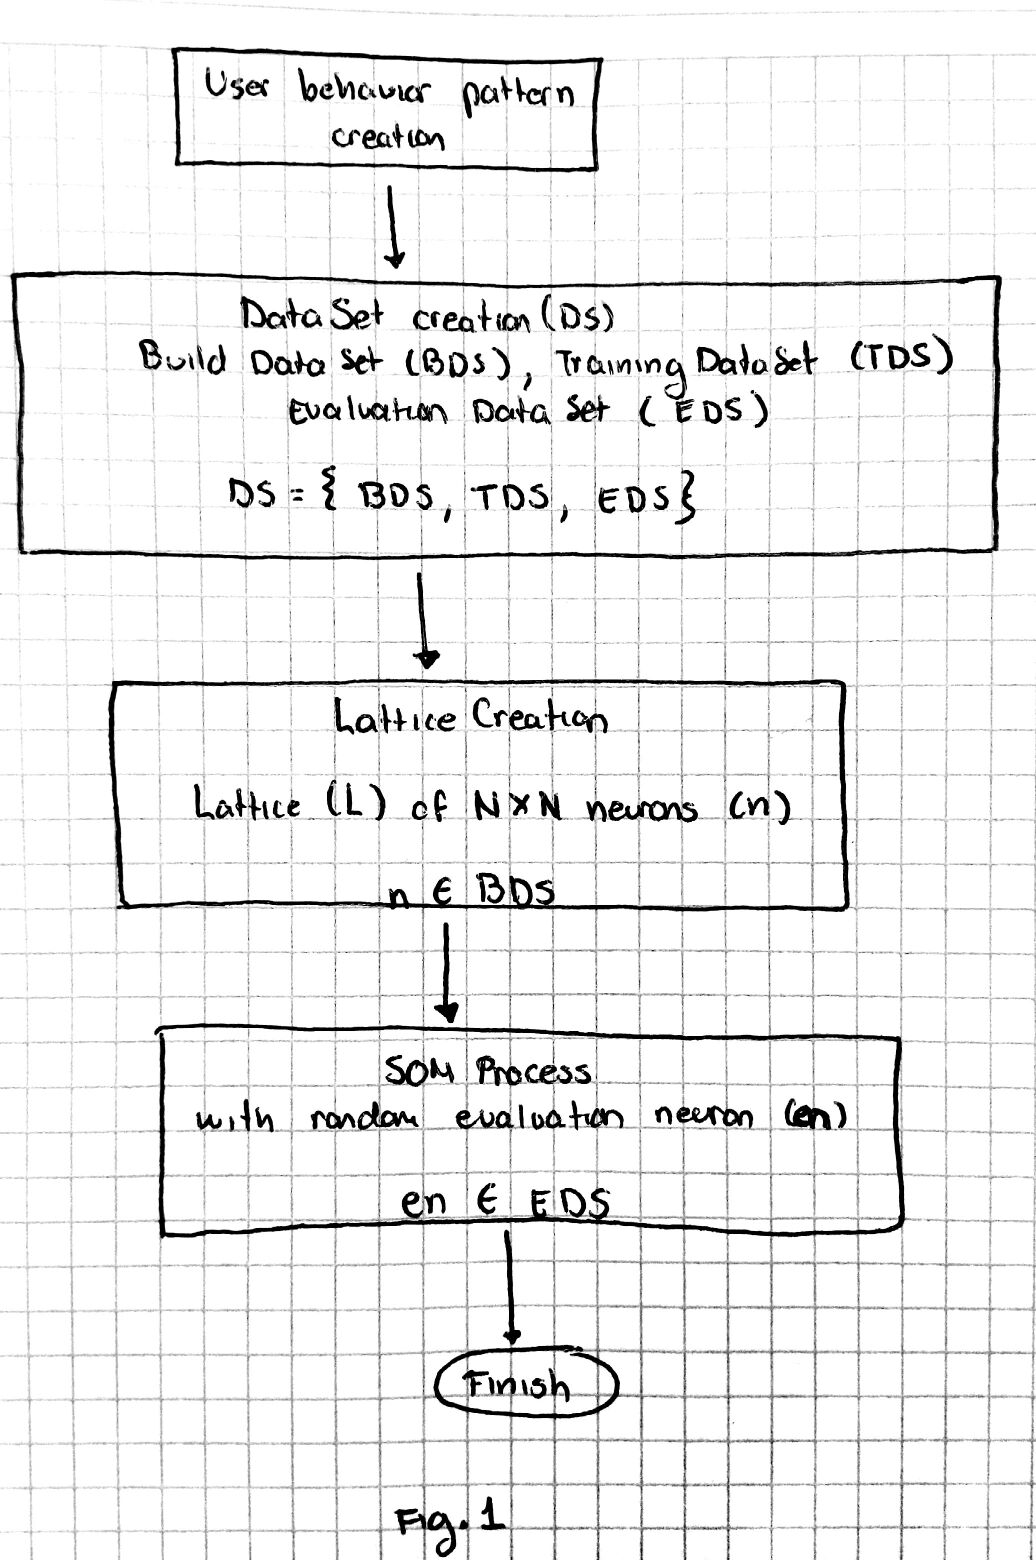
\includegraphics[scale=0.5]{fig-one} \end{center}

\subsubsection{SOM implementation} % level 3
For SOM implementation one layer square matrix of 100 x 100 neurons is used. As explained on section 4.0.1 each neuron has an individual feature vector, with specific weights. Our selected vector is conformed by three features, which summarize the total information sent in a range of time $\Delta$t over the network. For winner neuron evaluation euclidean distance is used. Winner and neighbor neurons weights are updated by a gaussian function.
using random initialization

\subsection{Experiment execution} % level 2
The experiment has the goal of verifying if the behavior of an user in the network can be addressed as a pattern, and use it to determine if the activity in the network belongs to it, or not. Experiment is divided in four parts: data collecting, user activity processing into data chunks for data set creation, lattice training through SOM algorithm and obtained pattern evaluation. Fig. 2 shows the complete process.

\begin{center}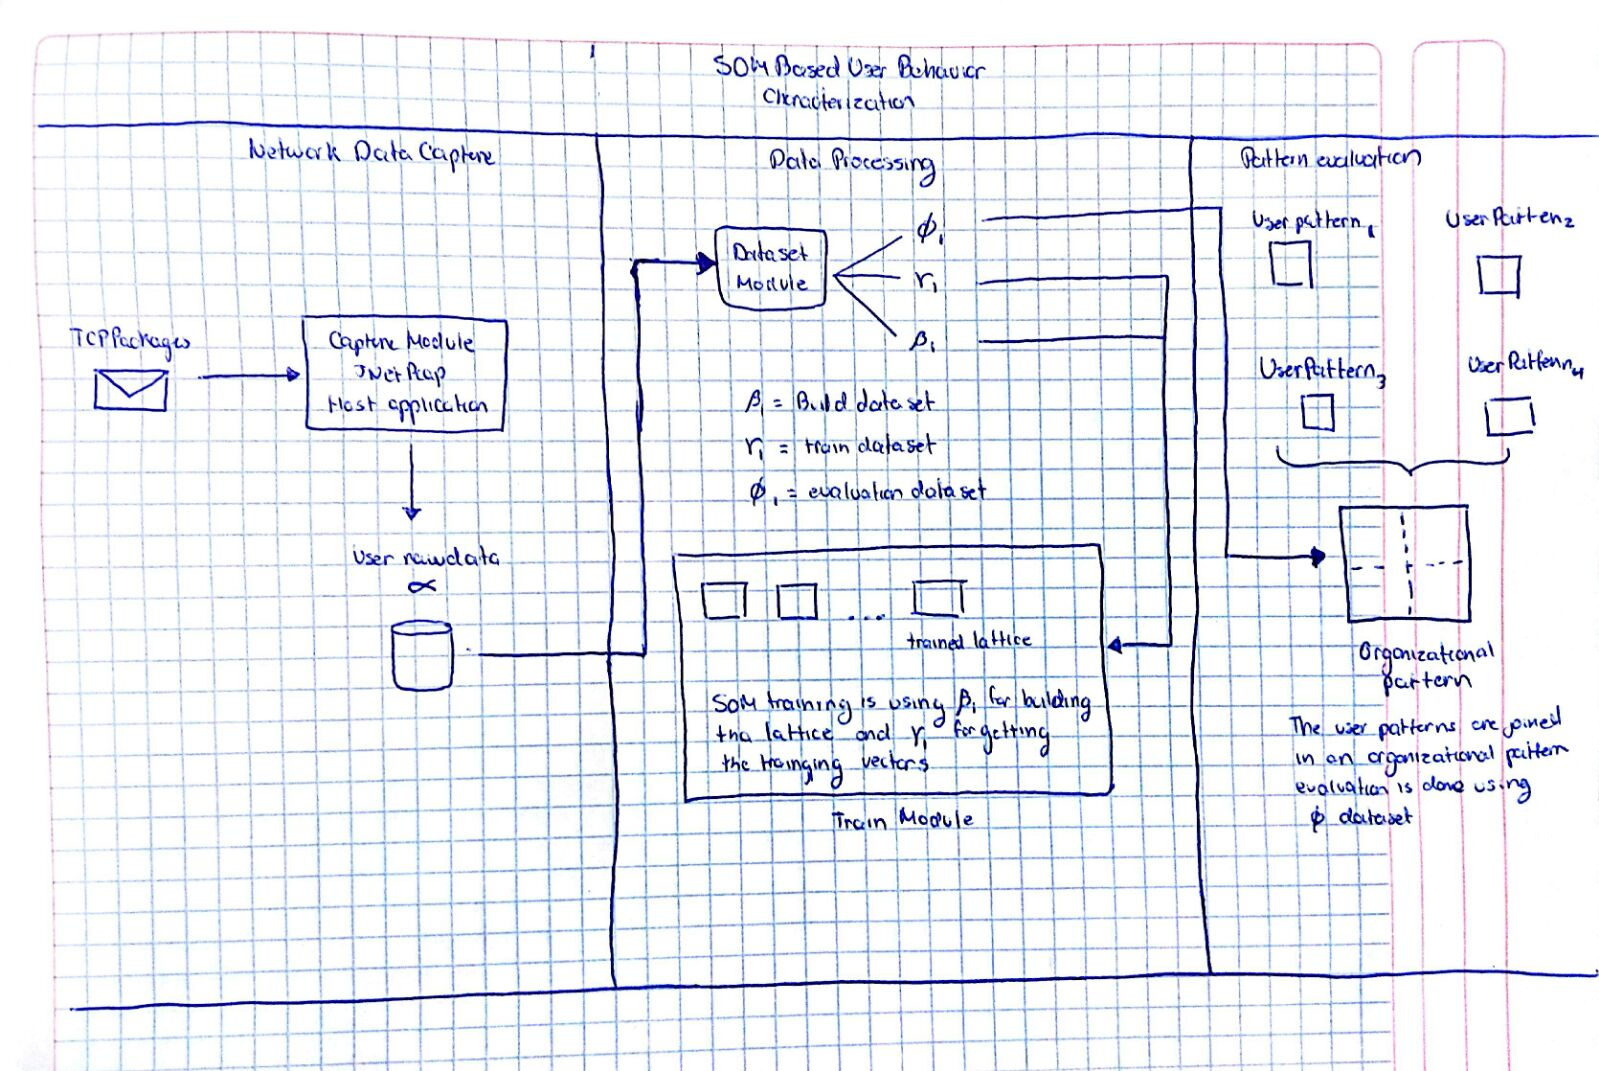
\includegraphics[scale=0.2]{fig-two} \end{center}

\subsubsection{Data collecting} % level 3
During two labor weeks,  network traffic was captured from each user's computer, it's important to say that only the owner has access to the computer. Before starting to capture, we checked that no computers had any malicious software installed. The average size of the captured traffic is 3 gigabytes per user, involving more than four million packets. Each network connection is characterized by eight parameters and specified as a eight-dimensional vector, organized as follows: way, origin IP, destination IP, used protocol, local used port, remote used port, total transmitted bytes and timestamp.

\subsubsection{Data Set creation} % level 3
Using packet as the unit for data evaluation is not an option due the great volume, and time consuming for processing \textbf{citation}, instead data is divided equally in three different types of datasets, one for building, other for training and the last for evaluation and then processed into data chunks. Fig 3 shows dataset creation.

\begin{center}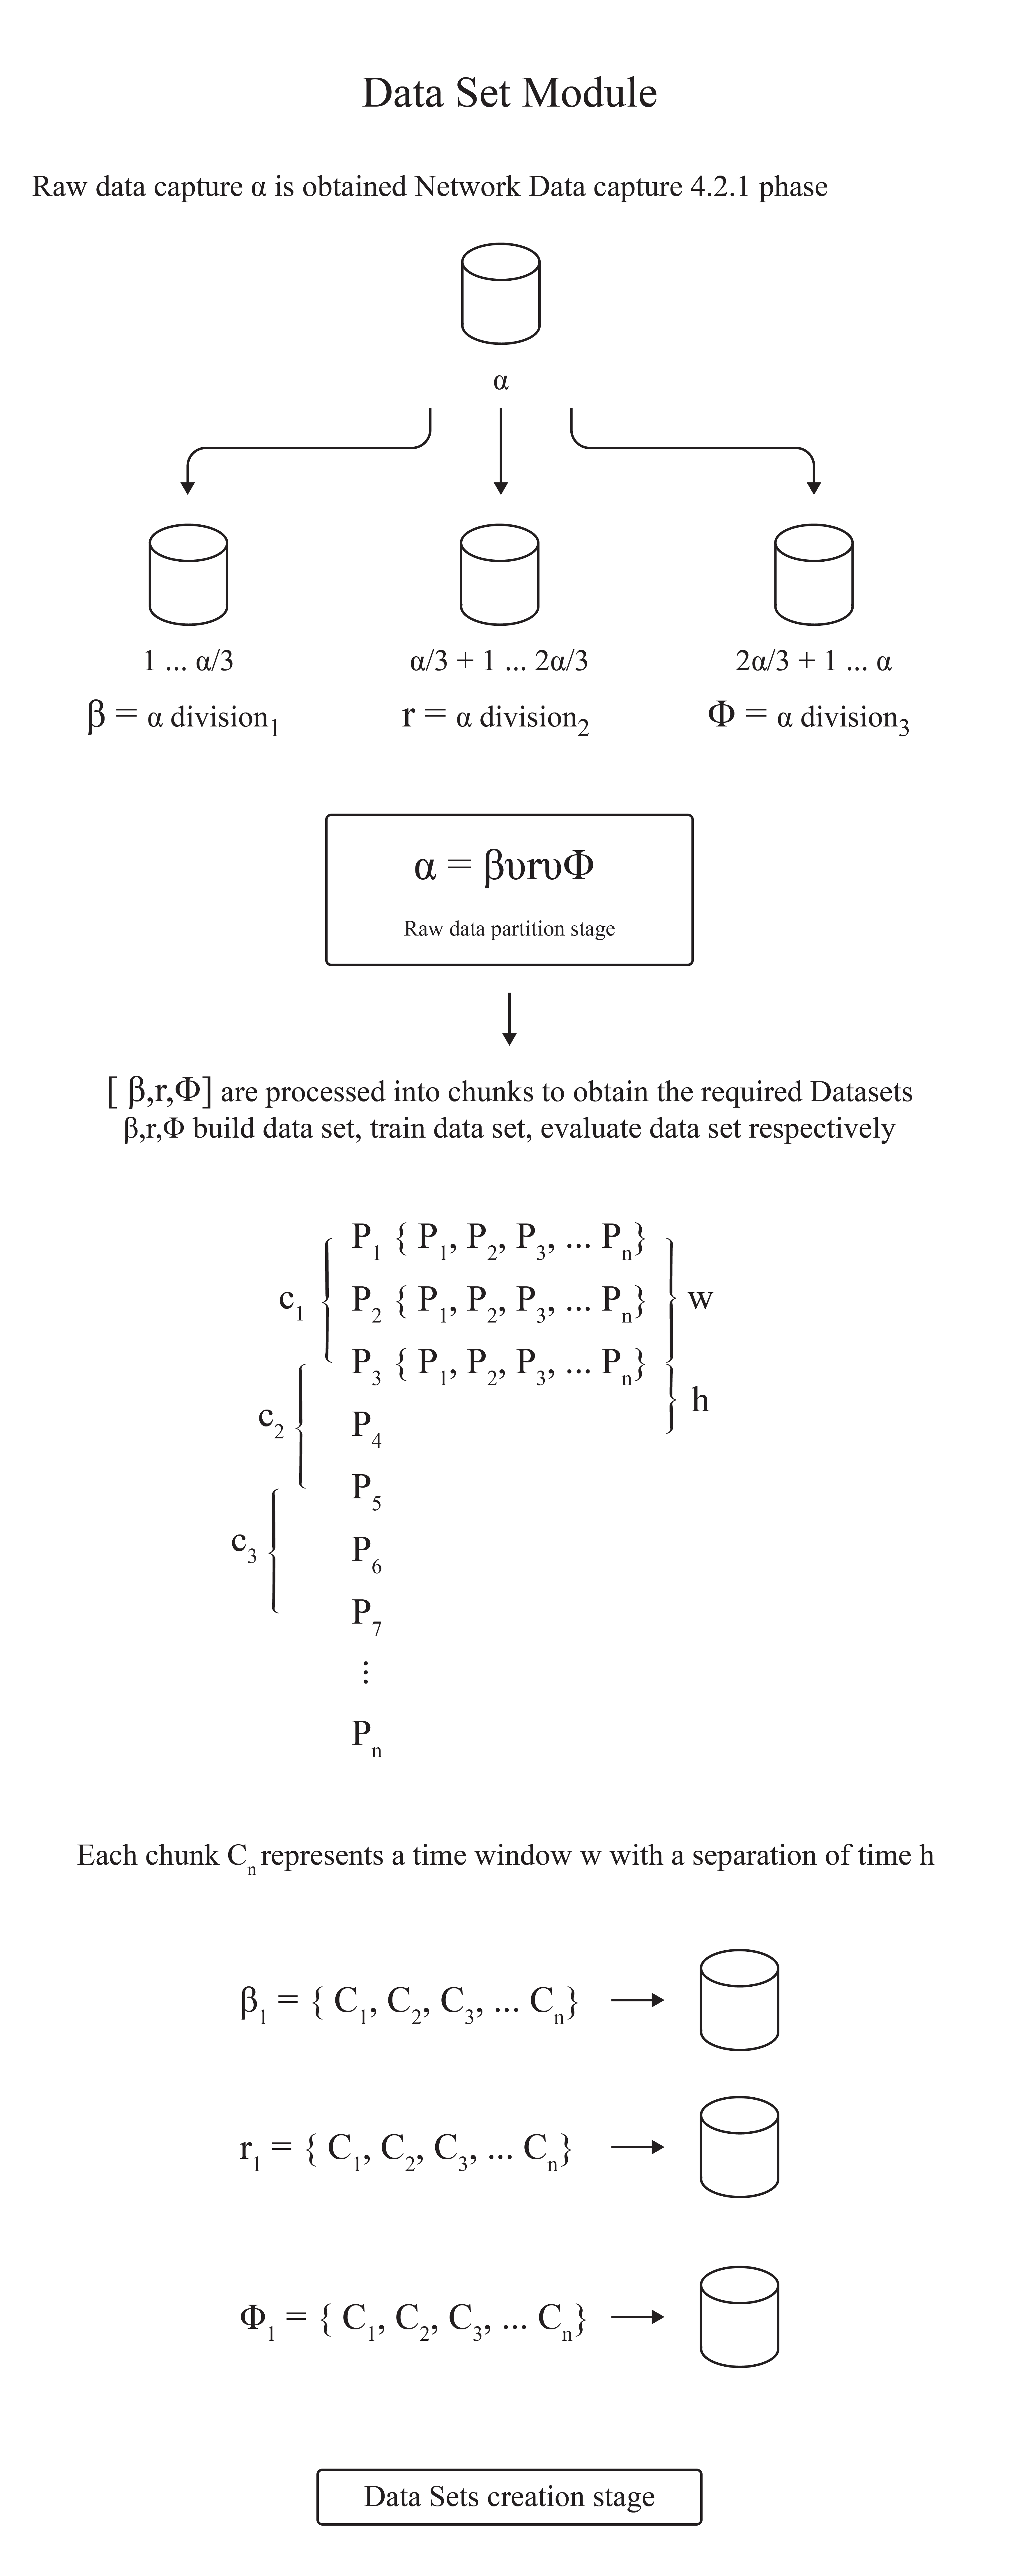
\includegraphics[scale=0.2]{fig-three} \end{center}

Each data set is created by 1...N data chunks. A data chunk has a set of continuous captured packages P1... P(N) which represents a fixed time window tw of five minutes measured by the packet timestamp, in which three metrics are obtained: a) TCP/UDP metric, represents the ratio between total bytes sent through both protocols and total bytes sent in the chunk b) bytes to Internal IP metric, represents the ratio between total bytes sent to CAN proxy ip and total bytes sent in the chunk and c) web traffic metric, represents the ratio between data sent through web ports, and and total bytes sent in the chunk. This metrics will be the features which SOM algorithm will arrange the clusters. After tw is processed, a time interval ti of 10 seconds is given to start the data chunk process creation until no more packages are available. Each dataset is conformed by XXX data chunks.

\subsubsection{SOM training} % level 3
This phase creates a user network pattern that represents its behavior in the network. Many pattern instances could be created from the user build dataset, as elements for creating it are randomly selected. Each neuron of the lattice is represented by an element of the Build Data Set, in which features are the three mentioned metrics in section 5.3.2. The lattice is has an arrange of 100 x 100 neurons, and a stop condition if 10 epochs.

---{Paper [1] ANDSOM Module - Training}

\subsubsection{Obtained pattern evaluation} % level 3
Comparison between two different lattices of the same user
Comparison between different lattices of multiple users



\section{Results and Discussion} % level 1
Results presentation, how the results are interpreted, and what we can do with data.
The results will explain, how the user is able to recognize itself in the organization map.

\section{Conclusions} % level 1

\subsection{Future work} % level 2
Due hardware limitation, SOM training is done with ten epochs. A much longer training of about one thousand epochs would give a more precise user pattern, helping in a better user detection in the organization map.
Also formulas are not completely following the standard of a gaussian function so a new implementation would be great.



\section{Bibliography} % level 1
[1] Ramadas, M., Ostermann, S.,  Tjaden, B. Detecting Anomalous Network Traffic with Self-organizing Maps.
[8] Dozono, H., Itou, S., and Nakakuni, M. (2007). Comparison of the adaptive authentication systems for behavior biometrics using the variations of self organizing maps. International Journal of Computers and Communications, 1(4), 108-116.
[25] T.Kohonen. Self Organizing Maps. Springer, third edition, 2001.



\end{document}